% Requires \usepackage{graphicx}. Adjust paths if included from another directory.
\begin{figure*}[t]
  \centering
  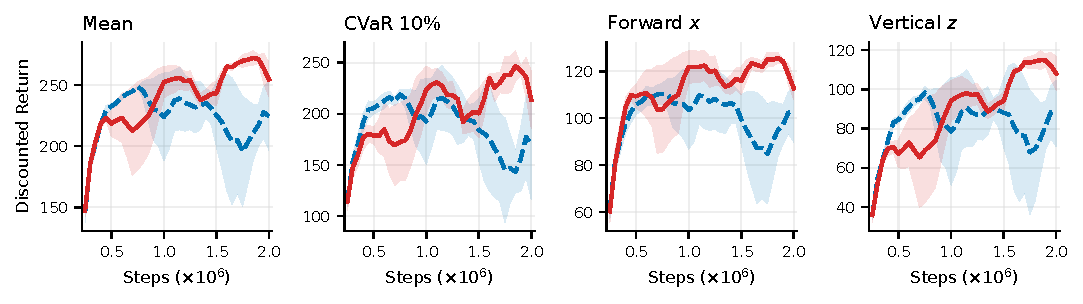
\includegraphics[width=0.95\textwidth]{paper/figures/hopper_5eval_four_panel.pdf}
  \par\smallskip
  
\includegraphics[width=0.30\textwidth]{paper/figures/hopper_5eval_legend.pdf}
  \caption{Hopper-v5 results for Uniform and D-LEVER. Panels show mean task return, CVaR$_{10}$, discounted forward-velocity reward, and discounted vertical-distance reward. The vertical reward uses ten times the distance from the origin. Each point averages five evaluations spaced 50,000 environment steps apart. Curves show the mean over seeds available for both methods; bands show one standard error across those seeds. Task returns are interquartile means across evaluation episodes, and CVaR$_{10}$ is the lowest return among ten fixed tasks. Four paired seeds contribute through 1.70 million steps and three from 1.75 to 2.00 million steps.}
  \label{fig:hopper-five-eval}
\end{figure*}
